%%%%%%%%%%%%%%%%%%%%%%%%%%% asme2ej.tex %%%%%%%%%%%%%%%%%%%%%%%%%%%%%%%
% Template for producing ASME-format journal articles using LaTeX    %
% Written by   Harry H. Cheng, Professor and Director                %
%              Integration Engineering Laboratory                    %
%              Department of Mechanical and Aeronautical Engineering %
%              University of California                              %
%              Davis, CA 95616                                       %
%              Tel: (530) 752-5020 (office)                          %
%                   (530) 752-1028 (lab)                             %
%              Fax: (530) 752-4158                                   %
%              Email: hhcheng@ucdavis.edu                            %
%              WWW:   http://iel.ucdavis.edu/people/cheng.html       %
%              May 7, 1994                                           %
% Modified: February 16, 2001 by Harry H. Cheng                      %
% Modified: January  01, 2003 by Geoffrey R. Shiflett                %
% Use at your own risk, send complaints to /dev/null                 %
%%%%%%%%%%%%%%%%%%%%%%%%%%%%%%%%%%%%%%%%%%%%%%%%%%%%%%%%%%%%%%%%%%%%%%

%%% use twocolumn and 10pt options with the asme2ej format
\documentclass[twocolumn,10pt]{asme2ej}

\usepackage{graphicx} %% for loading jpg figures
\usepackage{hyperref}   % to set up hyperlinks
\hypersetup{
	colorlinks=true,
	linkcolor=blue,
	citecolor=blue,
	urlcolor=blue,
}
\usepackage[square,numbers]{natbib}

%% The class has several options
%  onecolumn/twocolumn - format for one or two columns per page
%  10pt/11pt/12pt - use 10, 11, or 12 point font
%  oneside/twoside - format for oneside/twosided printing
%  final/draft - format for final/draft copy
%  cleanfoot - take out copyright info in footer leave page number
%  cleanhead - take out the conference banner on the title page
%  titlepage/notitlepage - put in titlepage or leave out titlepage
%
%% The default is oneside, onecolumn, 10pt, final


\title{A Novel Passive Ferrofluid One-way (Check) Valve}

%%% first author
\author{Veronica Stuckey
  \affiliation{
    Biomedical Engineer, University of Texas at Austin \\
    Email:  stuckey002@gmail.com
    }
}

%%% second author
%%% remove the following entry for single author papers
%%% add more entries for additional authors
\author{Robert L. Read
\affiliation{
  Founder, Public Invention\\
  Email: read.robert@gmail.com
    }
}

%%% third author
%%% remove the following entry for single author papers
%%% add more entries for additional authors

\begin{document}

\maketitle

%%%%%%%%%%%%%%%%%%%%%%%%%%%%%%%%%%%%%%%%%%%%%%%%%%%%%%%%%%%%%%%%%%%%%%
\begin{abstract}

Small pumps and valves enable flow management in microfluidic systems.
This paper presents a novel passive ferrofluid check valve.
The valve consists of only a
unique channel-and-chamber geometry, ferrofluid, and a stationary
magnetic field.
The flow is determined only by the inlet and output pressure,
and the magnetic field is completely static.
The prototype valve and experimental setup are explained
and performance of the valves cracking and collapse pressure reported.
This initial design can be used for microfluid handling and lab-on-a-chip
applications.
\end{abstract}

%%%%%%%%%%%%%%%%%%%%%%%%%%%%%%%%%%%%%%%%%%%%%%%%%%%%%%%%%%%%%%%%%%%%%%
\section{Introduction}

Ferrofluid can be manipulated by electronically controlled magnetic
fields to exert force on fluids\cite{torres2014recent,kole2021engineering,ozbey2015modeling}.
This makes it possible to build pneumatic or hydraulic
devices, perhaps on very small scales,
such as a single chip\cite{yamahata2003ferrofluid,hatch2001ferrofluidic}, to
miniaturize fluid handling.
This has been proposed for biomedical purposes\cite{michelson2019novel}
that would use water or body fluids,
although this paper reports only on experiments done with air.
Miniature pumps and valves could be used to make a “lab on a chip” (LOC) or
even to heat or cool different areas.
A fundamental component of such
devices is the check or one-way valve.
Two check
valves on either side of a chamber whose volume can vary creates a
positive displacement pump.
A perfect check valve opens or
{\em cracks} with minimal pressure on the inlet side and sustains maximal
pressure on the outlet side before {\em collapse},
allowing fluid to flow in only one
direction. Following\cite{hartshorne2004ferrofluid} we call the maximum pressure
differential the valve can resist in the direction it is intended to
check (from outlet to inlet) the {\em sustainable} or {\em collapse} pressure.

This article is a brief report on an initial but functioning design of a
passive ferrofluid check valve (PFCV) that has no moving
parts except for the ferrofluid bolus itself, which is stationary
in normal operation.
By passive, the authors
mean a check valve that functions without changes to the magnetic
field affecting the bolus, whether that field is induced by a
permanent magnet or an electromagnet.
That is, the flow is determined
purely by the difference between the inlet port pressure and the
outlet port pressure.
(This terminology is not completely standardized,
for example \cite{hartshorne2004ferrofluid} uses the
term {\em active} to simply mean a valve that is not a permanent seal.)
To our knowledge, no passive
ferrofluid check valve has been previously reported, despite being an
active area of research and despite such a valve having
significant advantages for operation but especially
fabrication over valves with moving parts.

%%%%%%%%%%%%%%%%%%%%%%%%%%%%%%%%%%%%%%%%%%%%%%%%%%%%%%%%%%%%%%%%%%%%%%
\section{Related Research}

A number of papers report on ferrofluid pumps, focusing in particular
on micropump and lab-on-a-chip applications\cite{ozbey2015modeling,hsu2018biocompatible}.
Many of these papers use
a version of mechanical valve not based on passive
ferrofluid, even though they move a ferrofluid bolus
with a magnetic field.
For example,
a corrugated silicone micro valve\cite{yamahata2003ferrofluid,yamahata2005plastic}
has been reported.
Other researchers use active valves, which require synchronization with
the ferrofluid plug to form a pump,
such as \cite{menz2000fluidic}, which
describes an active T-Valve with a moving ferrofluid plug, and
\cite{ando2009ferrofluidic} describes a complete fluid pump with valves
that use
active control of a ferrofluid bolus.
Active control is possible because the
action of the plunger or bolus may be synchronized with the opening and closing
of the valves.
Nonetheless a passive valve would be simpler and less
expensive, and would not require knowledge of the timing of the
plunger.
At least two additional kinds of active valves, a {\em well valve} and Y valve, have
been described\cite{hartshorne2004ferrofluid}.

A passive ferrofluid two-way valve with tunable
opening and closing pressure based on magnetic
field strength\cite{paschalis2013novel} has been tested,
but could not be passively used to make a pump.

This paper has not studied the closing pressure of the PFCV, but reports on
the opening (or cracking) pressure (for flow from inlet to outlet) and
sustainable (or collapse) pressure
when the outlet pressure is higher than the inlet side.
An interesting functional micropump in which the
moving ferrofluid bolus merges with a fixed ferrofluid valve and then
separates on each pumping cycle has been described\cite{hatch2001ferrofluidic},
but is not a one-way valve.

\section{Passive Ferrofluid Check Valve (PFCV) Design}
%%%%%%%%%%%%%%%% begin figure %%%%%%%%%%%%%%%%%%%
%%% 3.34in is the maximum width you can have for a figure
\begin{figure}
\centerline{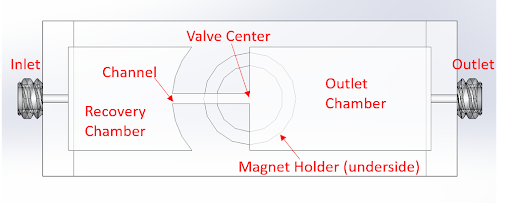
\includegraphics[width=3.34in]{figure/components.png}}
\caption{The passive ferrofluid check valve components}
\label{fig_components}
\end{figure}
%%%%%%%%%%%%%%%% end figure %%%%%%%%%%%%%%%%%%%

The PFCV depicted in Figure~\ref{fig_components} is a simple asymmetric volume
centered in a magnetic field
which holds a ferrofluid bolus in place.
In the center of a radially symmetric magnetic field
a narrow channel meets a larger open chamber at a right angle.
The ferrofluid bolus is large enough that at rest in the field it
forms a semi-circle in the open chamber. The narrow channel is
longer than the radius of the bolus at rest.
The broad chamber is the outlet side of the valve.
The narrow chamber opens onto a recovery chamber on the inlet
side of the valve.
This design allows the bolus to be recovered from the recovery
chamber when the pressure is equalized if the outlet pressure is
raised above the collapse pressure, driving the bolus away
from the magnetic field.
The PFCV does not resist pressure as well  as a
valve of the same size
made out of moving, solid parts.
That is, the sustainable
pressure it can resist on the outlet side before failing is relatively
low, and pressure required to crack it open and allow flow is
relatively high.
However, it may operate reliably within a range of
known pressures, and thus be sufficient to build a
pump-on-a-chip.
Furthermore, the PFCV reported here is a preliminary design which
can probably be significantly improved.
The authors found the
existence of the PFCV exciting enough to report on it immediately.

\section{Method}

The valve depicted Figure~\ref{fig_components}
was designed using Solidworks 2016.
It is freely licensed via the CERN OHL Strong Reciprocal License\cite{stuckey2021}.
The model consists of a 15mm long, 2mm wide and 2mm high channel,
two female luers, a magnet holder ring and two legs to provide room
for the magnet.  All volumes are 2mm high.
The 3D shape
of the chambers can be thought as a 2mm extrusion of a 2D shape.
Viewed from the top, one end opens up to a recovery
chamber of circular profile 30mm in diameter and the other
an outlet chamber with a flat wall.
A magnet holder ring 12.7mm inner diameter (1/2'') was created centered on the channel-chamber
junction, below where the bolus is placed, to hold a permanent magnet in place
at the center of the valve. When two magnets are used, the magnet on
top naturally stays in the same position due to attraction to the magnet below.
On the inlet side the channel
opens into a recovery chamber shaped to allow the ferrofluid to be
passively drawn back into the channel by the magnetic field after a
collapse of the bolus.
The model was printed on a Projet MJP 2500 (3D
Systems, Rock Hill, SC), using Visijet M2G-CL and VisiJet M2 SUP as
material and support respectively (3D Systems, Rock Hill, SC). Support
material was removed by using an EasyClean system (3D Systems, Rock
Hill, SC) and Dawn dish soap (Procter \& Gamble, Cincinnati, OH) to
remove residuals.


%%%%%%%%%%%%%%%% begin figure %%%%%%%%%%%%%%%%%%%
%%% 3.34in is the maximum width you can have for a figure
\begin{figure}
\centerline{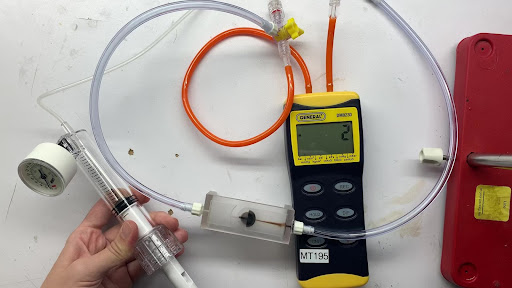
\includegraphics[width=3.34in]{figure/equipment.jpeg}}
\caption{Equipment set up}
\label{fig_equipment}
\end{figure}
%%%%%%%%%%%%%%%% end figure %%%%%%%%%%%%%%%%%%%

As shown in Figure~\ref{fig_equipment},
a basixCOMPAK 30atm pressurizing syringe (Merit Medical, South Jordan,
UT) is connected to the model via a two-way stopcock (Qosina,
Ronkonkoma, NY), tubing (Natvar, City of Industry, CA), and male
(Injectech, Fort Collins, CO) and female luer (Qosina, Ronkonkoma,
NY), allowing integration of a manometer (General Tools, Secaucus, NJ)
to measure pressure. A 12.7mm x 25.4mm (1/2” x 1”)
cylindrical neodymium magnet (Apex
Magnets, Petersburg, WV) with a pull force of 14.6 kg (32.24 pounds)
was placed inside the magnet channel by means
of a tight fit and 0.4 mL of ferrofluid (Apex Magnets, Petersburg, WV)
was injected into the model using a 3mL syringe (BH Supplies, Jackson,
NJ).

To obtain values, pressure was applied through the pressurizing
syringe, as demonstrated in a video \cite{stuckey2021video}.
Pressure was first applied from the outlet side of the model.
The maximum pressure difference from the outlet side the
valve can withstand before collapsing, will be referred to as the
sustainable pressure or {\em collapse} pressure.
Pressure applied from the inlet needed to
initiate flow will be referred to as the {\em cracking} pressure.

The cracking pressure was first measured by increasing the pressure
difference on the inlet side until flow is initiated (at which point
pushing the syringe plunger faster simply increases flow without
increasing the pressure.) Then the
collapse pressure was measured by increasing the pressure
difference on the outlet side. At pressures below the sustainable
pressure, the valve holds pressure well with no observable leaks of
air in the short time (a few minutes) of our experiment. When the
sustainable pressure is exceeded, the bolus explodes violently into
the recovery chamber. When the pressure difference is equalized, the
bolus may passively recover into the central position, or it may need
to be actively “combed” with a magnet back into the central position.

The procedure was performed first with one magnet, named the “Single
Magnet” configuration, placed below the channel-chamber connection.
The “Dual Magnet” configuration was performed with the magnet in the
same position as the Single Magnet case in the same position, but with
a second magnet of equal one placed vertically on top of the model,
arranged to be strongly attracted to the lower magnet.

\section{Results}
The final pressures obtained demonstrate a clear difference between
the inlet cracking pressure and outlet sustainable pressure, creating
an effective passive check valve.

%%%%%%%%%%%%%%% begin table   %%%%%%%%%%%%%%%%%%%%%%%%%%
\begin{table}[t]
\footnotesize
\caption{Result pressures}
\begin{center}
\label{table_ASME}
\begin{tabular}{|p{0.3in} |p{0.4in} |p{0.49in} |p{0.45in} |p{0.6in} |}
\hline
Magnet configuration &
Cracking Pressure kPa  (mmHg) &
Collapse Pressure kPa  (mmHg) &
Pressure Difference kPa  (mmHg) &
Approx. Ratio: Cracking to Collapse Pressure \\
\hline
Single &
1.1 (8) &
5.5 (41) &
4.4 (33) &
1:5 \\
\hline
Dual &
8.5 (64) &
17.5 (131)&
8.9 (67)&
1:2 \\
\hline
\end{tabular}
\end{center}
\end{table}
%%%%%%%%%%%%%%%% end table %%%%%%%%%%%%%%%%%%%


The ferrofluid had observable differences in behavior between the two
configurations.  After the pressure equalized
following a collapse of the bolus due to
exceeding the sustainable pressure, the single magnet
configuration often repaired itself by drawing the fluid back
into a centered bolus passively.
After a collapse with two magnets, fluid further from the bolus
remained stationary while the fluid closer was pulled back to the
center. Following the removal of the top magnet, the stationary fluid
then began to return to the bolus. This is consistent with the
localization of the magnetic field between two magnets, and the
weakening of the magnetic field further from the channel-chamber
juncture in the dual magnet configuration.

Although the dual magnet configuration demonstrated a larger absolute
pressure difference due to magnet strength between the
cracking and the collapse pressure, the single magnet configuration
granted a larger ratio of collapse pressure to cracking
pressure due to the much lower cracking pressure.
The authors conjecture that the low cracking pressure may have
been not only to the weaker magnetic field, but the weakening at the
top of the 2mm high channel, which was further away from the magnet
in the single magnet configuration.

\section{Conclusions}

This paper demonstrates an apparently novel passive ferrofluid one-way
valve or check valve (PFCV). This valve is completely passive in that
it depends entirely on the pressure at the inlet port and the outlet
port. The valve has no moving parts (except for the ferrofluid, which
is almost stationary), and a remarkably simple design, consisting of
nothing but a channel, an inlet chamber, and outlet chamber,
and a bolus of ferrofluid in a
static magnetic field.

Although no effort has been made to optimize the design, the pressure
difference between the cracking pressure and the sustainable back
pressure appear great enough to make an effective micropump. The
performance of this one-way valve may improve with additional design
effort; the authors sought to publish this result as soon as it was
observed.  Obvious future research possibilities are:
\begin{enumerate}
\item  To improve the
performance by varying the geometry of the passive design or shape and
strength of the magnetic field.
\item Utilizing this design to make a micro-pump
similar to earlier micro-pumps but with this simpler check valve
design.
\item To provide an explanatory and predictive theory of operation,
for example based on magnetic field strength as per \cite{ando2009ferrofluidic}.
\item Studying the ability of the valve to recover after
  a collapse automatically when high outlet pressure is removed,
  which would increase robustness in some applications.
\end{enumerate}

%%%%%%%%%%%%%%%%%%%%%%%%%%%%%%%%%%%%%%%%%%%%%%%%%%%%%%%%%%%%%%%%%%%%%%
% The bibliography is stored in an external database file
% in the BibTeX format (file_name.bib).  The bibliography is
% created by the following command and it will appear in this
% position in the document. You may, of course, create your
% own bibliography by using thebibliography environment as in
%
% \begin{thebibliography}{12}
% ...
% \bibitem{itemreference} D. E. Knudsen.
% {\em 1966 World Bnus Almanac.}
% {Permafrost Press, Novosibirsk.}
% ...
% \end{thebibliography}

% Here's where you specify the bibliography style file.
% The full file name for the bibliography style file
% used for an ASME paper is asmems4.bst.
\bibliographystyle{asmems4}

% Here's where you specify the bibliography database file.
% The full file name of the bibliography database for this
% article is asme2e.bib. The name for your database is up
% to you.
\bibliography{asme2e}

\end{document}

%%%%%%%%%%%%%%%%%%%%%%%%%%%%%%%%%%%%%%%%%%%%%%%%%%%%%%%%%%%%%%%%%%%%%%
\appendix       %%% starting appendix
\section*{Appendix A: Head of First Appendix}
Avoid Appendices if possible.

%%%%%%%%%%%%%%%%%%%%%%%%%%%%%%%%%%%%%%%%%%%%%%%%%%%%%%%%%%%%%%%%%%%%%%
\section*{Appendix B: Head of Second Appendix}
\subsection*{Subsection head in appendix}
The equation counter is not reset in an appendix and the numbers will
follow one continual sequence from the beginning of the article to the very end as shown in the following example.
\begin{equation}
a = b + c.
\end{equation}

%%%%%%%%%%%%%%%%%%%%%%%%%%%%%%%%%%%%%%%%%%%%%%%%%%%%%%%%%%%%%%%%%%%%%%
\subsection{Second-Level Heading}

The next level of heading is also boldface with upper and lower case letters.
The heading is flushed left with the left margin. The spacing to the next heading is two line spaces.

%%%%%%%%%%%%%%%%%%%%%%%%%%%%%%%%%%%%%%%%%%%%%%%%%%%%%%%%%%%%%%%%%%%%%%
\subsubsection{Third-Level Heading.}

The third-level of heading follows the style of the second-level heading.


%%%%%%%%%%%%%%%%%%%%%%%%%%%%%%%%%%%%%%%%%%%%%%%%%%%%%%%%%%%%%%%%%%%%%%
\section{Use of SI Units}

An ASME paper should use SI units.  When preference is given to SI units, the U.S. customary units may be given in parentheses or omitted. When U.S. customary units are given preference, the SI equivalent {\em shall} be provided in parentheses or in a supplementary table.

%%%%%%%%%%%%%%%%%%%%%%%%%%%%%%%%%%%%%%%%%%%%%%%%%%%%%%%%%%%%%%%%%%%%%%
\section{Footnotes\protect\footnotemark}
\footnotetext{Examine the input file, asme2ej.tex, to see how a footnote is given in a head.}

Footnotes are referenced with superscript numerals and are numbered consecutively from 1 to the end of the paper\footnote{Avoid footnotes if at all possible.}. Footnotes should appear at the bottom of the column in which they are referenced.


%%%%%%%%%%%%%%%%%%%%%%%%%%%%%%%%%%%%%%%%%%%%%%%%%%%%%%%%%%%%%%%%%%%%%%
\section{Mathematics}

Equations should be numbered consecutively beginning with (1) to the end of the paper, including any appendices.  The number should be enclosed in parentheses and set flush right in the column on the same line as the equation.  An extra line of space should be left above and below a displayed equation or formula. \LaTeX\ can automatically keep track of equation numbers in the paper and format almost any equation imaginable. An example is shown in Eqn.~(\ref{eq_ASME}). The number of a referenced equation in the text should be preceded by Eqn.\ unless the reference starts a sentence in which case Eqn.\ should be expanded to Equation.

\begin{equation}
f(t) = \int_{0_+}^t F(t) dt + \frac{d g(t)}{d t}
\label{eq_ASME}
\end{equation}

%%%%%%%%%%%%%%%%%%%%%%%%%%%%%%%%%%%%%%%%%%%%%%%%%%%%%%%%%%%%%%%%%%%%%%
\section{Figures}
\label{sect_figure}

All figures should be positioned at the top of the page where possible.  All figures should be numbered consecutively and centered under the figure as shown in Fig.~\ref{figure_ASME}. All text within the figure should be no smaller than 7~pt. There should be a minimum two line spaces between figures and text. The number of a referenced figure or table in the text should be preceded by Fig.\ or Tab.\ respectively unless the reference starts a sentence in which case Fig.\ or Tab.\ should be expanded to Figure or Table.


%%%%%%%%%%%%%%%%%%%%%%%%%%%%%%%%%%%%%%%%%%%%%%%%%%%%%%%%%%%%%%%%%%%%%%
%%%%%%%%%%%%%%%% begin figure %%%%%%%%%%%%%%%%%%%
\begin{figure}[t]
\begin{center}
\setlength{\unitlength}{0.012500in}%
\begin{picture}(115,35)(255,545)
\thicklines
\put(255,545){\framebox(115,35){}}
\put(275,560){Beautiful Figure}
\end{picture}
\end{center}
\caption{The caption of a single sentence does not have period at the end}
\label{figure_ASME}
\end{figure}
%%%%%%%%%%%%%%%% end figure %%%%%%%%%%%%%%%%%%%
%%%%%%%%%%%%%%%%%%%%%%%%%%%%%%%%%%%%%%%%%%%%%%%%%%%%%%%%%%%%%%%%%%%%%%

In the following subsections, I have inserted figures that have been provided by authors in order to demonstrate what to avoid.  In each case the authors provided figures that are 3.25in wide and 600dpi in the .tif graphics format.  The papers containing these figures have been held from production due to their poor quality.

%%%%%%%%%%%%%%%%%%%%%%%%%%%%%%%%%%%%%%%%%%%%%%%%%%%%%%%%%%%%%%%%%%%%%%
\subsection{The 1st Example of Bad Figure}

%%%%%%%%%%%%%%%% begin figure %%%%%%%%%%%%%%%%%%%
%%% 3.34in is the maximum width you can have for a figure
\begin{figure}
\centerline{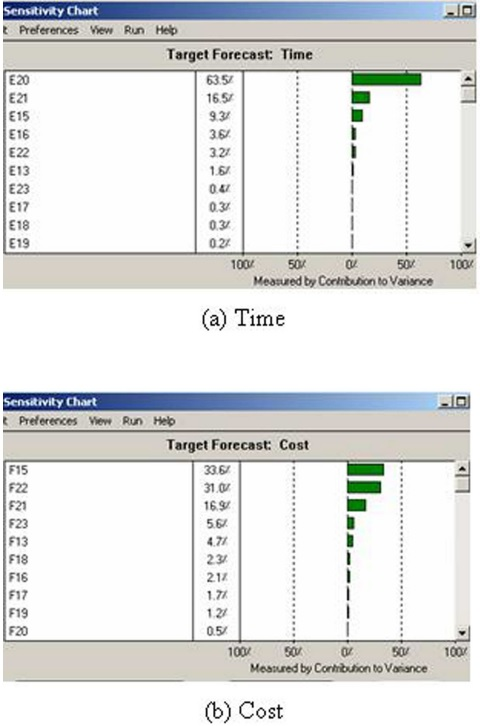
\includegraphics[width=3.34in]{figure/FMANU_MD_05_1107_11.jpg}}
\caption{Example taken from a paper that was held from production because the image quality is poor.  ASME sets figures captions in 8pt, Helvetica Bold.}
\label{fig_example1.jpg}
\end{figure}
%%%%%%%%%%%%%%%% end figure %%%%%%%%%%%%%%%%%%%

In order to place the figure in this template using MSWord, select Insert Picture from File, and use wrapping that is top and bottom. Make sure the figure is 3.25in wide.

Figure~`\ref{fig_example1.jpg}
was taken from a recent paper that was held from publication, because the text is fuzzy and unreadable. It was probably obtained by taking a screen shot of the computer output of the authors software. This means the original figure was 72dpi (dots per inch) on a computer screen. There is no way to improve the quality such a low resolution figure.

In order to understand how poor the quality of this figure is, please zoom in slightly, say to 200\%.  Notice that while the font of the paper is clear at this size, the font in the figures is fuzzy and blurred.  It is impossible to make out the small symbol beside the numbers along the abscissa of the graph.  Now consider the labels Time and Cost. They are clearly in fonts larger that the text of the article, yet the pixilation or rasterization, associated with low resolution is obvious. This figure must be regenerated at higher resolution to ensure quality presentation.

The poor quality of this figure is immediately obvious on the printed page, and reduces the impact of the research contribution of the paper, and in fact detracts from the perceived quality of the journal itself.



%%%%%%%%%%%%%%%%%%%%%%%%%%%%%%%%%%%%%%%%%%%%%%%%%%%%%%%%%%%%%%%%%%%%%%
\subsection{The 2nd Example of Bad Figure}

%%%%%%%%%%%%%%%% begin figure %%%%%%%%%%%%%%%%%%%
\begin{figure}
\centerline{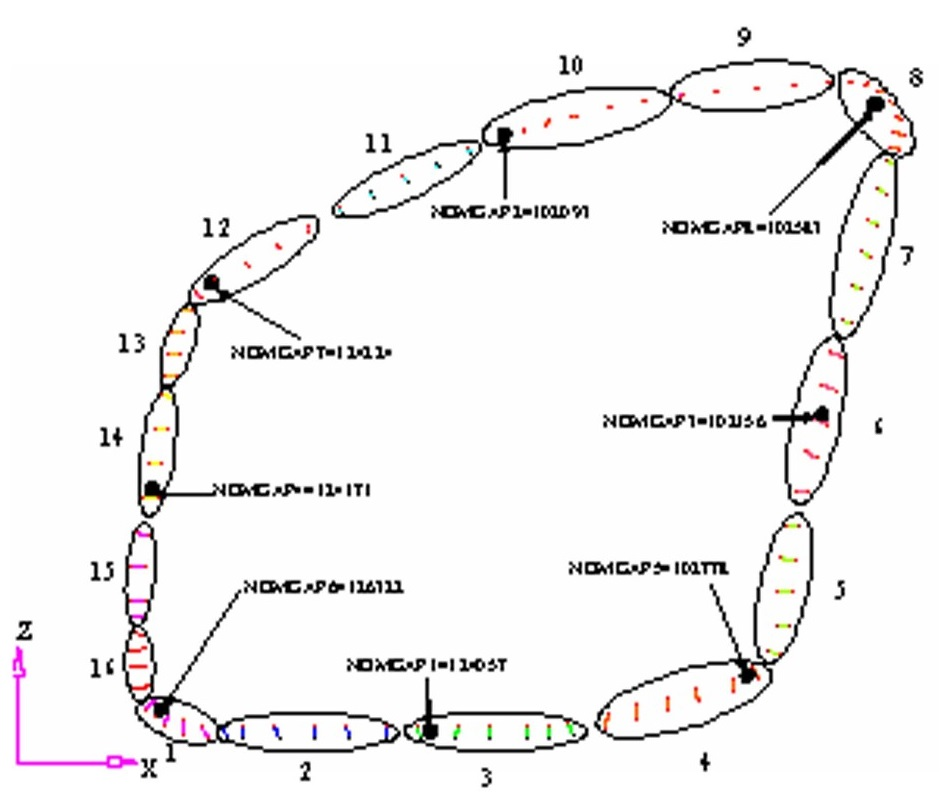
\includegraphics[width=3.34in]{figure/FMANU_MD_05_1272_5.jpg}}
\caption{While this figures is easily readable at a double column width of 6.5in, when it is shrunk to 3.25in column width the text is unreadable. This paper was held from production.}
\label{fig_}
\end{figure}
%%%%%%%%%%%%%%%% end figure %%%%%%%%%%%%%%%%%%%

Figure~\ref{fig_example2.jpg}
demonstrates a common problem that arises when a figure is scaled down fit a single column width of 3.25in.  The original figure had labels that were readable at full size, but become unreadable when scaled to half size.  This figure also suffers from poor resolution as is seen in the jagged lines the ovals that form the chain.

This problem can be addressed by increasing the size of the figure to a double column width of 6.5in, so the text is readable.  But this will not improve the line pixilation, and a large low resolution figure is less desirable than a small one.  This also significantly expands the length of the paper, and may cause it to exceed the JMD nine page limit.  Additional pages require page charges of \$200 per page.  It is best to regenerate the figure at the resolution that ensures a quality presentation.


%%%%%%%%%%%%%%%%%%%%%%%%%%%%%%%%%%%%%%%%%%%%%%%%%%%%%%%%%%%%%%%%%%%%%%
\subsection{The 3rd Example of Bad Figure}
%%%%%%%%%%%%%%%% begin figure %%%%%%%%%%%%%%%%%%%
\begin{figure}
\centerline{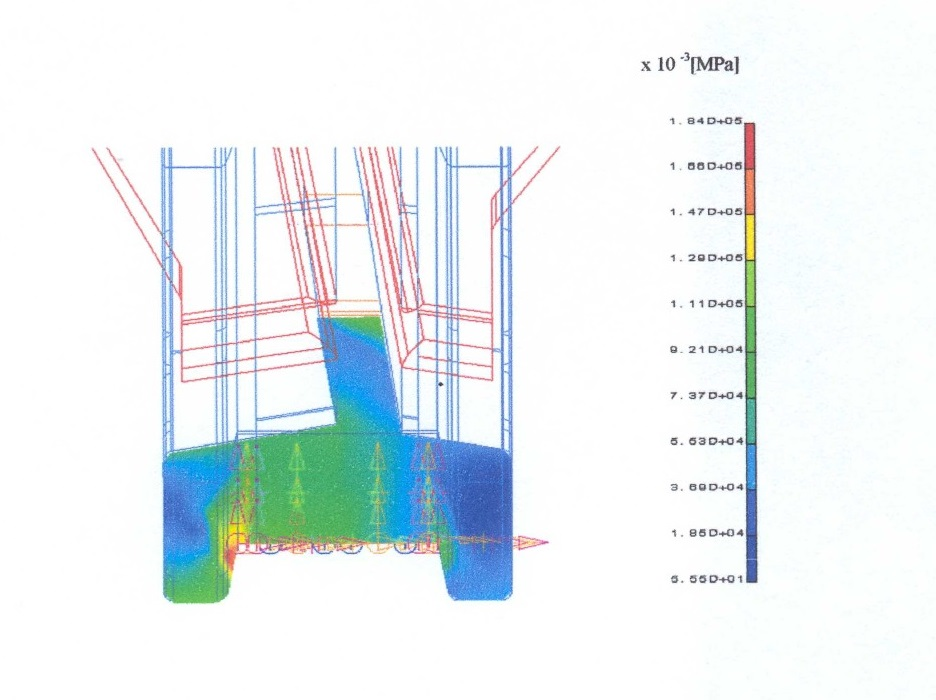
\includegraphics[width=3.25in]{figure/FMANU_MD_04_1274_13.jpg}}
\caption{Another example of a figure with unreadable text.  Even when the paper was expanded to double column width the text as shown in Fig.~\ref{fig_example4.jpg} was of such low quality that the paper was held from production.}
\label{fig_example3.jpg}
\end{figure}
%%%%%%%%%%%%%%%% end figure %%%%%%%%%%%%%%%%%%%

%%%%%%%%%%%%%%%% begin figure %%%%%%%%%%%%%%%%%%%
%%% the maximum width in double column is 6.85in
\begin{figure*}
\centerline{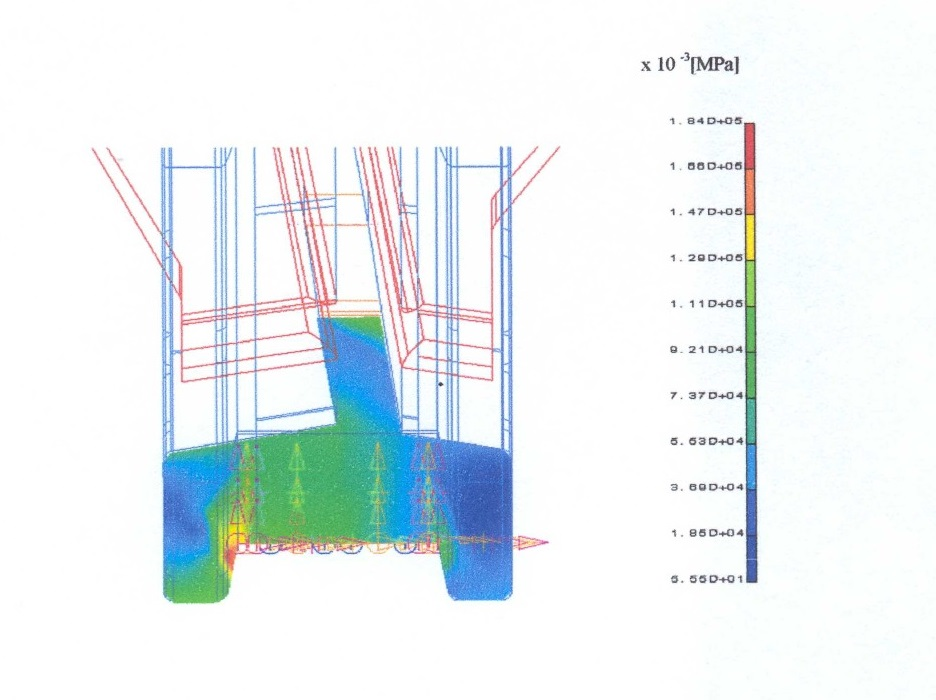
\includegraphics[width=6.85in]{figure/FMANU_MD_04_1274_13.jpg}}
\caption{A figure expanded to double column width the text from Figure~\ref{fig_example3.jpg}}
\label{fig_example4.jpg}
\end{figure*}
%%%%%%%%%%%%%%%% end figure %%%%%%%%%%%%%%%%%%%
An author provided the high resolution image
in Fig.~\ref{fig_example3.jpg}
that was sized to a single column width of 3.25in.  Upon seeing the poor quality of the text, the publisher scaled the image to double column width as shown in Fig.~\ref{fig_example4.jpg}
at which point it took half of a page.  The publisher went on to do this for all eight figures generating four pages of figures that the author did not expect. ASME stopped production of the paper even with the larger figures due to the pixilation of the font.

Clearly the text in this figure is unreadable, and it is doubtful that the author can print the output in a way that it is readable.  This is a problem that the author must solve, not the publisher.

As you might expect, I have many more examples, but in the end the author is the best judge of what is needed in each figure.  ASME simply requires that the image meet a minimum standard for font and line quality, specifically the font should be the appropriate size and not be blurred or pixilated, and that lines should be the appropriate weight and have minimal, preferably no, pixilation or rasterization.


%%%%%%%%%%%%%%%%%%%%%%%%%%%%%%%%%%%%%%%%%%%%%%%%%%%%%%%%%%%%%%%%%%%%%%
\section{Tables}

%%%%%%%%%%%%%%%%%%%%%%%%%%%%%%%%%%%%%%%%%%%%%%%%%%%%%%%%%%%%%%%%%%%%%%
%%%%%%%%%%%%%%%%%%%%%%%%%%%%%%%%%%%%%%%%%%%%%%%%%%%%%%%%%%%%%%%%%%%%%%

All tables should be numbered consecutively  and centered above the table as shown in Table~\ref{table_ASME}. The body of the table should be no smaller than 7 pt.  There should be a minimum two line spaces between tables and text.


%%%%%%%%%%%%%%%%%%%%%%%%%%%%%%%%%%%%%%%%%%%%%%%%%%%%%%%%%%%%%%%%%%%%%%
\section{Citing References}

%%%%%%%%%%%%%%%%%%%%%%%%%%%%%%%%%%%%%%%%%%%%%%%%%%%%%%%%%%%%%%%%%%%%%%
The ASME reference format is defined in the authors kit provided by the ASME.  The format is:

\begin{quotation}
{\em Text Citation}. Within the text, references should be cited in  numerical order according to their order of appearance.  The numbered reference citation should be enclosed in brackets.
\end{quotation}

The references must appear in the paper in the order that they were cited.  In addition, multiple citations (3 or more in the same brackets) must appear as a `` [1-3]''.  A complete definition of the ASME reference format can be found in the  ASME manual \cite{asmemanual}.

The bibliography style required by the ASME is unsorted with entries appearing in the order in which the citations appear. If that were the only specification, the standard {\sc Bib}\TeX\ unsrt bibliography style could be used. Unfortunately, the bibliography style required by the ASME has additional requirements (last name followed by first name, periodical volume in boldface, periodical number inside parentheses, etc.) that are not part of the unsrt style. Therefore, to get ASME bibliography formatting, you must use the \verb+asmems4.bst+ bibliography style file with {\sc Bib}\TeX. This file is not part of the standard BibTeX distribution so you'll need to place the file someplace where LaTeX can find it (one possibility is in the same location as the file being typeset).

With \LaTeX/{\sc Bib}\TeX, \LaTeX\ uses the citation format set by the class file and writes the citation information into the .aux file associated with the \LaTeX\ source. {\sc Bib}\TeX\ reads the .aux file and matches the citations to the entries in the bibliographic data base file specified in the \LaTeX\ source file by the \verb+\bibliography+ command. {\sc Bib}\TeX\ then writes the bibliography in accordance with the rules in the bibliography .bst style file to a .bbl file which \LaTeX\ merges with the source text.  A good description of the use of {\sc Bib}\TeX\ can be found in \cite{latex, goosens} (see how two references are handled?).  The following is an example of how three or more references \cite{latex, asmemanual,  goosens} show up using the \verb+asmems4.bst+ bibliography style file in conjunction with the \verb+asme2ej.cls+ class file. Here are some more \cite{art, blt, ibk, icn, ips, mts, mis, pro, pts, trt, upd} which can be used to describe almost any sort of reference.

%%%%%%%%%%%%%%%%%%%%%%%%%%%%%%%%%%%%%%%%%%%%%%%%%%%%%%%%%%%%%%%%%%%%%%
\section{Conclusions}
The only way to ensure that your figures are presented in the ASME Journal of Mechanical Design in the way you feel is appropriate and meets the requirement for quality presentation is for you to prepare a double column version of the paper in a form similar to that used by the Journal.

This gives you the opportunity to ensure that the figures are sized appropriately, in particular that the labels are readable and match the size of the text in the journal, and that the line weights and resolutions have no pixilation or rasterization.  Poor quality figures are immediately obvious on the printed page, and this detracts from the perceived quality of the journal.

I am pleased to provide advice on how to improve any figure, but this effort must start with a two-column version of the manuscript. Thank you in advance for your patience with this effort, it will ensure quality presentation of your research contributions.



%%%%%%%%%%%%%%%%%%%%%%%%%%%%%%%%%%%%%%%%%%%%%%%%%%%%%%%%%%%%%%%%%%%%%%
\section{Discussions}
This template is not yet ASME journal paper format compliant at this point.
More specifically, the following features are not ASME format compliant.
\begin{enumerate}
\item
The format for the title, author, and abstract in the cover page.
\item
The font for title should be 24 pt Helvetica bold.
\end{enumerate}

\noindent
If you can help to fix these problems, please send us an updated template.
If you know there is any other non-compliant item, please let us know.
We will add it to the above list.
With your help, we shall make this template
compliant to the ASME journal paper format.


%%%%%%%%%%%%%%%%%%%%%%%%%%%%%%%%%%%%%%%%%%%%%%%%%%%%%%%%%%%%%%%%%%%%%%
\begin{acknowledgment}
ASME Technical Publications provided the format specifications for the Journal of Mechanical Design, though they are not easy to reproduce.  It is their commitment to ensuring quality figures in every issue of JMD that motivates this effort to have authors review the presentation of their figures.

Thanks go to D. E. Knuth and L. Lamport for developing the wonderful word processing software packages \TeX\ and \LaTeX. We would like to thank Ken Sprott, Kirk van Katwyk, and Matt Campbell for fixing bugs in the ASME style file \verb+asme2ej.cls+, and Geoff Shiflett for creating
ASME bibliography stype file \verb+asmems4.bst+.
\end{acknowledgment}

%%%%%%%%%%%%%%%%%%%%%%%%%%%%%%%%%%%%%%%%%%%%%%%%%%%%%%%%%%%%%%%%%%%%%%
\begin{nomenclature}
\entry{A}{You may include nomenclature here.}
\entry{$\alpha$}{There are two arguments for each entry of the nomemclature environment, the symbol and the definition.}
\end{nomenclature}
